\documentclass[12pt]{article}

\usepackage{xargs}
\usepackage[utf8]{inputenc}
\usepackage[margin=2cm]{geometry}
\usepackage[T2A]{fontenc}
\usepackage{csquotes}
\usepackage{tabulary}
\usepackage{graphicx}
\usepackage[capitalize]{cleveref}
%\usepackage[style=apa,block=ragged]{biblatex}
\usepackage[english]{babel}
\usepackage{verbatim}
\usepackage{amsmath}
\usepackage{systeme}
\usepackage{amssymb}
\usepackage{array}
\usepackage{listings}
\usepackage{xcolor}
\usepackage{siunitx}
\usepackage[section]{placeins}
%\addbibresource{main.bib}

\definecolor{codegreen}{rgb}{0,0.6,0}
\definecolor{codegray}{rgb}{0.5,0.5,0.5}
\definecolor{codepurple}{rgb}{0.58,0,0.82}
\definecolor{backcolour}{rgb}{0.95,0.95,0.92}

\lstdefinestyle{mystyle}{
    backgroundcolor=\color{backcolour},
    commentstyle=\color{codegreen},
    keywordstyle=\color{magenta},
    numberstyle=\tiny\color{codegray},
    stringstyle=\color{codepurple},
    basicstyle=\ttfamily\footnotesize,
    breakatwhitespace=false,
    breaklines=true,
    captionpos=b,
    keepspaces=true,
    numbers=left,
    numbersep=5pt,
    showspaces=false,
    showstringspaces=false,
    showtabs=false,
    tabsize=2
}


\lstset{style=mystyle}

\setlength{\parskip}{0.5em}

\title{Курсова Работа ЦРПСУ}
\author{Рафаел Калъчев 011217071}
\date{}

\newcommand\inputfile[1]{%
    \InputIfFileExists{#1}{}{\typeout{No file #1.}}%
}

\newcommand\includegraphicsifexists[2][width=\linewidth]{\IfFileExists{#2}{\includegraphics[#1]{#2}}{ \typeout{No file #2.}}}

\newcommand{\incfig}[3]{
	\begin{figure}[htbp!]
		\centering
		\includegraphics[width=0.6\textwidth]{#1}
		\caption{#2}
          	\label{#3}
	\end{figure}
}


\begin{document}

\maketitle

\section{Упражнение 1}

От зададената ни система:

\begin{equation}
	W(s) = \frac{2}{(6s+1)(12s+1)}
\end{euation

Създаваме модел в средата на матлаб. 
Изполсваме Симулинк за да изведем преходната характеристика 
на модела (фиг. \ref{fig:get_step}),
която ще изполваме за идентификация, 
чрез следните методи:  
Метод на Циглер-Николс, Метод на допирателната и Метод на Стрейц.

Използвайки получените двупараметрични и трипараметрични модели,
пристъпваме, към настройка на ПИД регулатори, 
използвайки следните методи:
Метод на Циглер-Николс-1, Метод на Коен-Куун, Метод на Чиен, Хронес и Резуик.
След получаване на настройките на регулаторите, 
използваме средата на симулинк, 
за да симулираме поведението на затворената система с всеки 
един от получените регулатори (фиг. \ref{fig:lab1_compare_pids}).

Сопълнителните функции и скриптове са публикувани в Апендикса.

\lstinputlisting[language=Octave, caption=Matlab скрипт Лабораторно упражнение 1]{src/lab1.m}

\lstinputlisting[language=Octave, caption=Резултати Лабораторно упражнение 1]{src/lab1.res}


\begin{figure}[htbp!]
	\centering
	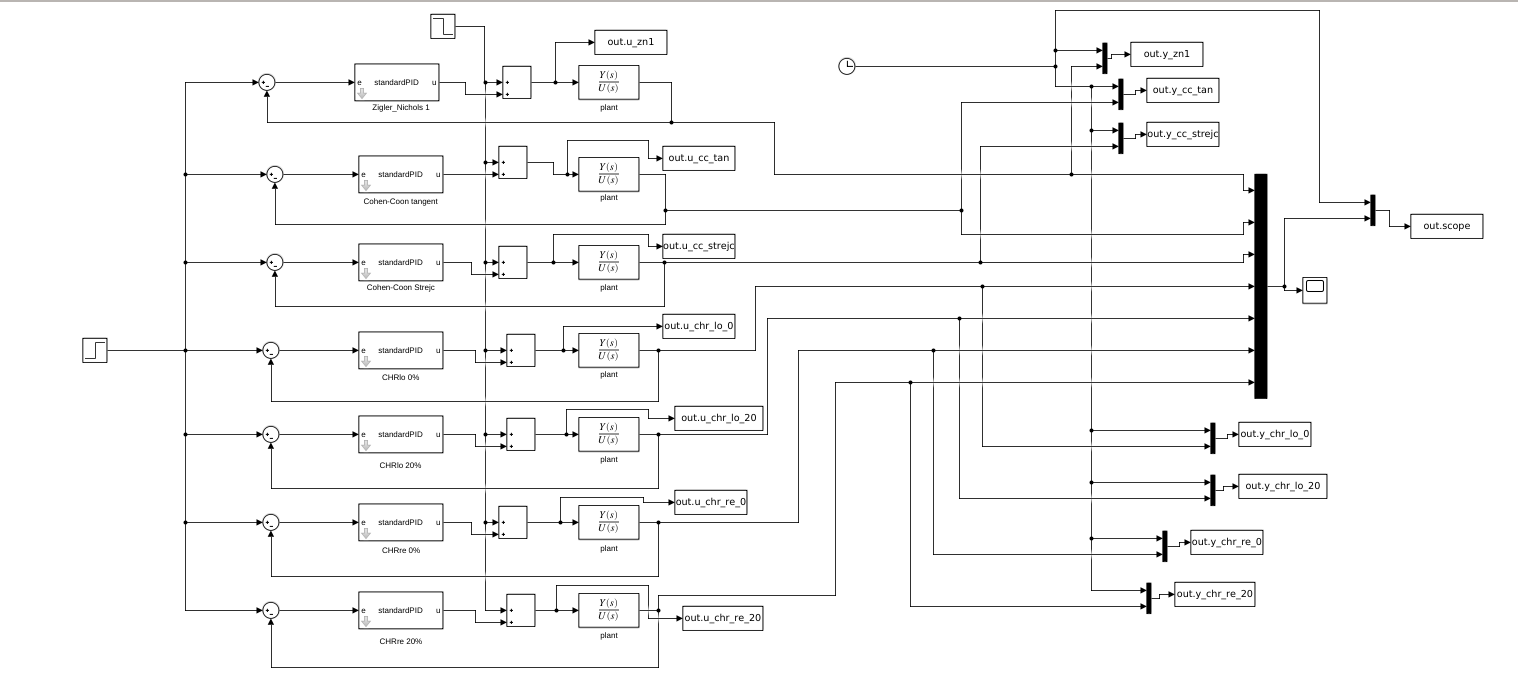
\includegraphics[width=0.9\textwidth]{img/lab1_compare_pids}
	\caption{Модел за съпоставка на всички регулатори}
	\label{fig:lab1_compare_pids}
\end{figure}

\incfig{img/lab1_get_step}{Симулинк Модел за снемане на преходната характеристика}{fig:get_step}

\incfig{h2aL_fig}{Снемане на параметри по метод на Циглер-Николс 1}{fig:lab1_zn1}

\incfig{h2KTL_fig}{Снемане на параметри по метод на допирателната}{fig:lab1_tangent}

\incfig{src/h2Strejc}{Снемане на параметри по метод на Стрейц}{fig:lab1_tangent}

\incfig{compare_tan_fig}{Сравнение на Зададената система с апроксимацията по метод на допирателната}{fig:compare_tangent}

\incfig{compare_strejc_fig}{Сравнение на Зададената система с апроксимацията по Метод на Стрейц}{fig:compare_strejc}

\incfig{compare_pids_u_fig}{Съпоставка на управляващото въздействие при различните настойки на ПИД}{fig:lab1_comapre_pids_u}

\incfig{compare_pids_y_fig}{Съпоставка на изхода при различните настойки на ПИД}{fig:lab1_compare_pids_y}

\incfig{img/industrial_pid}{Индустриален ПИД контролер}{fig:ind_pid}

\incfig{img/comapre_industrial}{Симулинк схема за съпоставке между стандатен и индустриален ПИД}{fig:ind_comp}

\incfig{img/industrial_fig.png}{Съпоставка между стандартен и индустриален ПИД}{fig:ind_comapare}

\subsection{Изводи}

Забелязваме, че пререгулирането пр всички контролери, 
освен тези получени с методи за следене на заданието 
и Метода на Стрейц имат прекалено голямо пререгулиране, 
но тези методи не се справят толкова добре с отработването
на смущения.

ПИД регулаторът, получен с методът на Стрейц има най-голямо време
за установяване.

Най-бързо при промяна на заданието се установява рекълаторът, проектиран
за следене на заданието с методът на  Чиен, Хронес и Резуик (20\%)


Заблеязваме, че има малки разлики между стандартният и индустиалнният ПИД по отношение ан управелнието.
Определено може да се забележи влошаване на качествата, на преходният процес, при използване на индустриалният ПИД (фиг. \ref{fig:ind_comapare})

\section{Упражнение 2}

В това упражнение, ще подобрим стандартният ПИД регулатор от Лабораторно упражнение 1,
като добавим anti-windup механисъм, и насишане на изхода.
И ще изследваме, как това се отразява на управлението.

структурите на 2та вида регулатори са показани на (фиг \ref{fig:std_pid_struct} и \ref{fig:better_pid_struct}  )

\incfig{img/lab1_standard_pid}{Блок стандартен ПИД регулатор}{fig:std_pid_struct}

\incfig{img/lab2_standard_pid_better}{Блок подобрен стандартен ПИД регулатор}{fig:better_pid_struct}

за изследването е създаден следният модел в средата на Симулинк 
(фиг \ref{fig:compare_spid_bspid})

\incfig{img/lab2_compare_pids.png}{Симулинк модел за съпоставка на стандартният и подобрен ПИД регулатори}{fig:compare_spid_bspid}


\lstinputlisting[language=Octave, caption=Лабораторно упражнение 2 скрипт]{src/lab2.m}

\lstinputlisting[language=Octave, caption=Резултати лабораторни упражнение 2]{src/lab2.res}

\incfig{src/compare_pv_spid_vs_bspid_fig}{Съпоставка на изходът на системата, при стандартен и подобрен ПИД}{fig:res_compare_pv_spid_bspid}

\incfig{src/compare_u_spid_vs_bspid_fig}{Съпоставка на управлеващото въздействие на стандартен и подобрен ПИД}{fig:res_compare_u_spid_bspid}


\subsection{Изводи}

Забелязваме, че в случай на насищане на изходът на конторлера интегралната съставка
продължава да се увеличава, и пходният процес се влошава драстично.
Когато нямаме насищане и anti-windup функцията са изключени тогава конторлерът се държи,
като стандартен ПИД.
За да се справим с проблемът с интеграторът, когато сме в режим на насищане
активираме anti-windup функционалностаа. Така характеристиките на преходният процес се подобрават.


\section{Упражнение 4}

\incfig{img/lab4_universal_pid}{Структура на Универсален ПИД}{fig:universal_pid_struct}
\incfig{img/lab4_compare_universal_kap_tau}{Симулинк модел за съпоставка на капа и тау методите}{fig:compare_kap_tau}
\incfig{img/lab4_pst_pid}{Симулинк модел за съпоставка между капа и тау методте, чрез П-С-Т дискретен ПИД}{fig:compare_pst_pid}
\incfig{img/lab4_pst_pid_struct}{Структура на П-С-Т дискретен ПИД}{fig:pst_pid_struct}


\lstinputlisting[language=Octave, caption=Лабораторнo упражнение 4 скрипт]{src/lab4.m}
\lstinputlisting[language=Octave, caption=Резултати лабораторнo упражнение 4]{src/lab4.res}

\incfig{src/compare_u_kap_tau}{Съпоставка на управляващото въздействие на Универсален ПИД настроен с капа и тау методи }{fig:comapre_u_kap_tau}

\incfig{src/compare_y_kap_tau}{Съпоставка на изходите, при управление с Универален ПИД настроен с капа и тау методи}{fig:comapre_y_kap_tau}

\subsection{Изводи}

Забелязвааме, че при използване на капа метода получаваме много по бтрзо установяване на системата.
Но това се дължи на агресивното поведение на конторлера. забелязваме, оф (фиг. \ref{fig:comapre_u_kap_tau}),
че контролера изпада в автоколебания, за да поддържа системата стабилна.
Това в повечето случаи е не желано поведение.

Също забелазваме, че капа и тау методите са значително по-добри от методите разгледани до сега. 
При тях получаваме по-бързо установяване на сиситемата, значително по-малко пререгулиране.



\section{Апендикс}

\lstinputlisting[language=Octave, caption=PIDtun\_CHRlo.m]{src/PIDtun_CHRlo.m}
\lstinputlisting[language=Octave, caption=PIDtun\_CHRre.m]{src/PIDtun_CHRre.m}
\lstinputlisting[language=Octave, caption=h2KTL.m]{src/h2KTL.m}
\lstinputlisting[language=Octave, caption=h2aL.m]{src/h2aL.m}
\lstinputlisting[language=Octave, caption=h2Strejc.m]{src/h2Strejc.m}
\lstinputlisting[language=Octave, caption=infl\_ind.m]{src/infl_ind.m}
\lstinputlisting[language=Octave, caption=max\_sigma.m]{src/max_sigma.m}
\lstinputlisting[language=Octave, caption=settle\_time.m]{src/settle_time.m}
\lstinputlisting[language=Octave, caption=square\_control\_deviation.m]{src/square_control_deviation.m}
\lstinputlisting[language=Octave, caption=square\_error.m]{src/square_error.m}
\lstinputlisting[language=Octave, caption=weighted\_square\_quality.m]{src/weighted_sqare_quality.m}
\lstinputlisting[language=Octave, caption=PIDtun\_AHkap.m]{src/PIDtun_AHkap.m}
\lstinputlisting[language=Octave, caption=PIDtun\_HAtau.m]{src/PIDtun_AHtau.m}

\lstinputlisting[language=Octave, caption=dpid\_PST.m]{src/dpid_PST.m}
\lstinputlisting[language=Octave, caption=dpid\_Uni.m]{src/dpid_Uni.m}
\end{document}
